\documentclass{article}

\usepackage{mathtools,amsfonts}
\usepackage{enumitem}
\usepackage{fullpage}
\usepackage{fancyvrb}
\usepackage{hyperref}
\usepackage{pgfplots}
\pgfplotsset{compat=1.15}
\usepackage{mathrsfs}
\usetikzlibrary{arrows}
\usepackage{parskip}

\begin{document}
\thispagestyle{empty}
\definecolor{wrwrwr}{rgb}{0.3803921568627451,0.3803921568627451,0.3803921568627451}

\begin{center} \Large \bfseries
  Advanced Test 3 Solutions
  \\ \vspace{1em}
  Stellenbosch Camp 2022
\end{center}

\bigskip

\begin{enumerate}[itemsep=24pt]

\item 
For acute triangle $\triangle ABC$, a point $Z$ interior to $\triangle ABC$ satisfies $ZB = ZC$.
Suppose points $X$ and $Y$ lie outside $\triangle ABC$ such that $\triangle XAB \mathrel{|||} \triangle YCA \mathrel{|||} \triangle ZBC$.
Prove that $A,X,Y,Z$ are the vertices of a parallelogram. 

\textbf{Solution:}
$$\angle ZCY = \angle ZCA + \angle ACY = \angle ZCA + \angle BCZ = \angle BCA \implies \frac{ZC}{BC} = \frac{YC}{AC} \qquad (\triangle ZCB \mathrel{|||} \triangle YCA).$$
Therefore $\triangle BCA \mathrel{|||} \triangle ZCY$ as the sides are proportional and they have a common angle. Similarly $\triangle BCA \mathrel{|||} \triangle BZX$. 

Since $BZ = ZC \implies \triangle BZX \equiv \triangle ZCY \implies XZ = YC = AY$ and $ZY = BX = XA$.
Therefore $AXZY$ is a parallelogram.


\item %
For nonzero real numbers $a$, $b$, and $c$, show that
\[ \frac{a}{b} +\frac{b}{c} +\frac{c}{a} = \frac{a}{c} +\frac{c}{b} +\frac{b}{a} \]
if and only if two of $a$, $b$, and $c$ are equal.

\textbf{Solution:} Observe the following computation:
\begin{align*}
  \frac{a}{b} +\frac{b}{c} +\frac{c}{a} &= \frac{a}{c} +\frac{c}{b} +\frac{b}{a} \\
  \iff 0 &= \frac{a}{b} +\frac{b}{c} +\frac{c}{a} -\frac{a}{c} -\frac{c}{b} -\frac{b}{a} \\
  &= \frac{a^{2}b + b^{2}c + c^{2}a}{abc} -\frac{a^{2}c + b^{2}a + c^{2}b}{abc} = \frac{a^{2}c + b^{2}a + c^{2}b -(a^{2}b + b^{2}c + c^{2}a)}{abc} \\
  &= \frac{abc + a^{2}c + b^{2}a + c^{2}b - (a^{2}b + b^{2}c + c^{2}a+abc)}{abc} \\
  &= \frac{(a-b)(b-c)(c-a)}{abc}.
\end{align*}
Thus the equation holds if and only if one of $a-b$, $b-c$, $c-a$ is zero, showing that some pair among $a$, $b$, $c$ must be equal.


\item % Tsimerman
Can you tile a $10\times 10\times 10$ cube with $4\times 1\times 1$ blocks? (Standard tiling rules apply---cover the whole volume, no overlaps, etc.)

\textbf{Solution:}
The answer is no. Consider the following colouring: there are 10 `layers' to the cube. Label these layers from 1 to 10. For layers 1,2,5,6,9,10, we colour the layer as follows:
\begin{center}
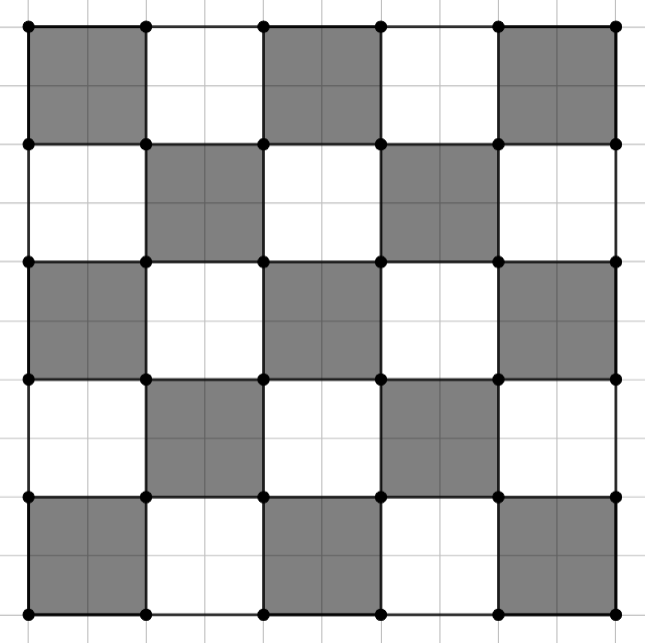
\includegraphics[scale=0.5]{Capture.png}
\end{center}
For layers 3,4,7,8, we invert these colours.
We note that each $4\times 1\times 1$ covers exactly 2 shaded blocks and 2 unshaded.
But counting the total number of shaded blocks gives 504, while there are 496 unshaded blocks.
Thus, we can not tile the shape as requested. 


\item % 
Consider an infinite sequence $(a_n)_{n=0}^{\infty}$ of positive integers such that for $n \geq 0$, we have that
\[
    a_{n + 1} = a_n + b_n
\]
where $b_n$ is the last (units) decimal digit of $a_n$. Show that the sequence contains infinitely many powers of $2$ if and only if $a_0$ is not a multiple of $5$.

\textbf{Solution:}
If $a_0$ is a multiple of 5, it will end in a 0 or 5 and be at least as big as 5. $a_1$ will then end in a 0, and the sequence becomes constant.

Assume $a_0$ is not a multiple of 5.
$a_1$ will end in an even digit.
We will now continue to cycle through the last digits $2\rightarrow 4 \rightarrow 8 \rightarrow 6$, whose sum is 20. Thus, we will obtain all numbers of the form $a_1+20k$.
We look at the last two digits of $2^n$ and note that they will repeat in the pattern $$\textbf{04}, 08, 16, 32, 64, 28, 56, 12, 24, 48, 96, 92, 84, 68, 36, 72, 44, 88, 76, 52, \textbf{04}, 08, ...$$

If the second last digit of $a_1$ is even and the last digit is 4 or 8, then we will obtain all powers of 2 ending in 4 or 8. If the second last digit is odd and the last digit is 2 or 6, we will obtain all powers of 2 ending in 2 or 6.

If $a_1$ ends in a 4, and the second last digit is odd, then $a_4$ will be $a_1+18$, which will end in a 2 and have the second last digit odd. We will now obtain all numbers of the form $a_4+20k$, which again gives infinite powers of 2.

If $a_1$ ends in a 8 and the second last digit is odd, then $a_3=a_1+14$ will end in a 2 and the second last digit will be odd. A similar argument applies.

If $a_1$ ends in a 2 and the second last digit is even, then $a_2=a_1+2$ ends in a 4 and the second last digit is even.

If $a_1$ ends in a 6 and the second last digit is even, then $a_2=a_1+6$ ends in a 2 and the second last digit is odd.


\item %  IMO Shortlist 1998 G3
Let $I$ be the incenter of triangle $\triangle ABC$.
Let $D$, $E$ and $F$ be the points of tangency of the incircle of $\triangle ABC$ with $BC$, $CA$ and $AB$, respectively.
The line $\ell$ passes through $B$ and is parallel to $DF$.
The lines $ED$ and $EF$ intersect $\ell$ at the points $X$ and $Y$.
Prove that $\angle XIY$ is acute.

\textbf{Solution:} 



\begin{center}
\begin{tikzpicture}[line cap=round,line join=round,>=triangle 45,x=0.3cm,y=0.3cm]
  \clip(-14,-18) rectangle (18,14);
  \draw [line width=1pt,color=wrwrwr] (-7.48418072213211,11.943124790001734)-- (9.851072169964434,-4.109768681891099);
  \draw [line width=1pt,color=wrwrwr] (9.851072169964434,-4.109768681891099)-- (-10.910046034501077,-4.1752906960620875);
  \draw [line width=1pt,color=wrwrwr] (-10.910046034501077,-4.1752906960620875)-- (-7.48418072213211,11.943124790001734);
  \draw [line width=1pt,color=wrwrwr] (-4.120771171316693,1.3403872874828022) circle (5.494223694538245);
  \draw [line width=1pt,color=wrwrwr] (-0.3877344450702902,5.371631612269011)-- (-4.103431507507615,-4.153809045165356);
  \draw [line width=1pt,color=wrwrwr,domain=-23.37794930246684:24.80881197642785] plot(\x,{(--109.10645878569908-9.525440657434366*\x)/-3.715697062437325});
  \draw [line width=1pt,color=wrwrwr,domain=-23.37794930246684:24.80881197642785] plot(\x,{(--50.04075544833976--2.8889978704593577*\x)/9.107212667095684});
  \draw [line width=1pt,color=wrwrwr,domain=-23.37794930246684:24.80881197642785] plot(\x,{(-49.627514715624955-6.636442786975009*\x)/5.391515604658359});
  \draw [line width=1pt,color=wrwrwr] (-4.120771171316693,1.3403872874828022)-- (15.51776782456035,10.417188783846877);
  \draw [line width=1pt,color=wrwrwr] (-4.120771171316693,1.3403872874828022)-- (5.312705659956814,-15.744178093192318);
  \draw [line width=1pt,color=wrwrwr] (-4.120771171316693,1.3403872874828022)-- (9.851072169964434,-4.109768681891099);
  \draw [line width=1pt,color=wrwrwr] (-4.120771171316693,1.3403872874828022)-- (-0.3877344450702902,5.371631612269011);
  \draw [line width=1pt,color=wrwrwr] (-4.120771171316693,1.3403872874828022)-- (-4.103431507507615,-4.153809045165356);

  \draw [fill=black] (-7.48418072213211,11.943124790001734) circle (1pt);
  \draw[color=black, left] (-7.48418072213211,11.943124790001734) node {$A$};
  \draw [fill=black] (9.851072169964434,-4.109768681891099) circle (1pt);
  \draw[color=black,right] (9.851072169964434,-4.109768681891099) node {$B$};
  \draw [fill=black] (-10.910046034501077,-4.1752906960620875) circle (1pt);
  \draw[color=black,left] (-10.910046034501077,-4.1752906960620875) node {$C$};
  \draw [fill=black] (-4.120771171316693,1.3403872874828022) circle (1pt);
  \draw[color=black,left] (-4.120771171316693,1.3403872874828022) node {$I$};
  \draw [fill=black] (-0.3877344450702902,5.371631612269011) circle (1pt);
  \draw[color=black,above] (-0.3877344450702902,5.371631612269011) node {$F$};
  \draw [fill=black] (-4.103431507507615,-4.153809045165356) circle (1pt);
  \draw[color=black,below left] (-4.103431507507615,-4.153809045165356) node {$D$};
  \draw [fill=black] (-9.494947112165974,2.4826337418096536) circle (1pt);
  \draw[color=black,below left] (-9.494947112165974,2.4826337418096536) node {$E$};
  \draw[color=black] (2.0,-20.0) node {$\ell$};
  \draw [fill=black] (15.51776782456035,10.417188783846877) circle (1pt);
  \draw[color=black,above left] (15.51776782456035,10.417188783846877) node {$Y$};
  \draw [fill=black] (5.312705659956814,-15.744178093192318) circle (1pt);
  \draw[color=black,right] (5.312705659956814,-15.744178093192318) node {$X$};
\end{tikzpicture}
\end{center}
Note that if  $\triangle XIY$ is acute then $\angle XIY$ is acute. So the problem can be reduced to proving that
\begin{flalign} %Keep this environment I need the equation annotation
  XI^2 +IY^2 > XY^2 \label{eqn:e1}.
\end{flalign}
We notice that $IF=ID$ (radii) and $BF=BD$ (tangents), thus $DIFB$ is a kite, thus $IB\perp FD$, thus $IB\perp XY$ (corresponding angles, $DF \parallel XY$). We can now reduce our proof requirement (\ref{eqn:e1})
\begin{flalign}
  && XI^2 +IY^2 &> XY^2 &\nonumber\\
  &\iff& XB^2+BI^2+BI^2+BY^2 &> (XB+BY)^2 & (\text{Pythagoras})\nonumber\\
  &\iff& XB^2+BY^2+2BI^2 &> XB^2+2XB \cdot BY+ BY^2 &\nonumber\\
  &\iff& BI^2 &> XB \cdot BY. &\label{eqn:e2}
\end{flalign}

Notice that $\angle BXD = \angle FDE = \angle AFE = \angle BFY$ (corresponding angles, tan-chord, vertically opposite respectively). Similarly we see $\angle BDX = \angle EDC = \angle EFD = \angle BYF$. Therefore $\triangle BDX \mathrel{|||} \triangle BYF$ (2 angles equal). This yields the equality of ratios
\begin{flalign*}
  &&\frac{XB}{BD} &= \frac{FB}{BY}& &\iff& XB \cdot BY &= FB \cdot BD = FB^2.&
\end{flalign*}
We deduce that
\begin{flalign*}
  XB \cdot BY = FB^2 = BI^2 - IF^2 < BI^2.
\end{flalign*}
So (\ref{eqn:e2}) is indeed satisfied.

\end{enumerate}

\end{document}
